\documentclass{article}
%color definitions
% \definecolor{ashgrey}{rgb}{0.7, 0.75, 0.71}
% \definecolor{bondiblue}{rgb}{0.0, 0.58, 0.71}
% \definecolor{blue(ryb)}{rgb}{0.01, 0.28, 1.0}
% \definecolor{byzantium}{rgb}{0.44, 0.16, 0.39} %morado
% \definecolor{darkgreen}{rgb}{0.0, 0.2, 0.13}
% \definecolor{darkspringgreen}{rgb}{0.09, 0.45, 0.27}
% \definecolor{dartmouthgreen}{rgb}{0.05, 0.5, 0.06}
% \definecolor{debianred}{rgb}{0.84, 0.04, 0.33}
% \definecolor{mygray}{rgb}{0.5,0.5,0.5}
% \definecolor{aurometalsaurus}{rgb}{0.43, 0.5, 0.5}
% \definecolor{asparagus}{rgb}{0.53, 0.66, 0.42}
% \definecolor{arylideyellow}{rgb}{0.91, 0.84, 0.42}
% \definecolor{brown(traditional)}{rgb}{0.59, 0.29, 0.0}
% \definecolor{brass}{rgb}{0.71, 0.65, 0.26}
% \definecolor{carrotorange}{rgb}{0.93, 0.57, 0.13}
% \definecolor{darkpastelblue}{rgb}{0.47, 0.62, 0.8}
% \definecolor{brandeisblue}{rgb}{0.0, 0.44, 1.0}

\usepackage[utf8]{inputenc}
\usepackage[binary-units]{siunitx}
\usepackage[shortcuts]{extdash}
\usepackage[margin=1.5cm]{geometry}
\usepackage[table,xcdraw]{xcolor}
\usepackage[printonlyused]{acronym} %for acronyms
\usepackage{hyperref} %para url
\hypersetup{
    colorlinks=true,
    linkcolor=blue,
    filecolor=magenta,      
    urlcolor=brandeisblue,
}
\usepackage{mathtools} % loads amsmath
\usepackage{textcomp} %\textregistered % or \textcopyright
\usepackage{soul} % para tachar texto con una linea e.g \st{texto tachado}
\usepackage{colortbl}
\usepackage{multicol}
\usepackage{multirow}
\usepackage{makecell}
\usepackage{hhline}
\usepackage{array}
\usepackage{graphicx}
\usepackage{caption}
\usepackage{lscape}
\usepackage{afterpage}
\usepackage{pgf}
\usepackage{cleveref} %for references
%music packages
\usepackage{musicography}
\usepackage{stackengine}
%%para escribir codigo en LaTeX
\usepackage{soul} %% to enable highlight a una linea de codigo
\usepackage{listings,lstautogobble}[showlines=htrue,breakatwhitespace=true] 
\lstloadlanguages{C}
\lstset{ %language=[Sharp]C, %necesario para el emphasize,
basicstyle=\fontfamily{pcr}\selectfont\footnotesize\color{black},
keywordstyle=\color{blue(ryb)}\bfseries, % style for keywords
commentstyle=\color{dartmouthgreen}\ttfamily,
stringstyle=\color{brown(traditional)}\ttfamily, %procnamestyle=\color{brown(traditional)}\ttfamily
%morecomment=[l][\color{brass}]{\#include},
%morecomment=[l][\color{brass}]{\#define},
%morecomment=[s][\color{brown(traditional)}]{/´}{´},
morecomment=*[l][\special@on\color{dartmouthgreen}\itshape]{//},
morecomment=*[s][\special@on\color{dartmouthgreen}\itshape]{/*}{*/},
%morecomment=*[n][\special@on\color{darkpastelblue}]{(0x}{x0)},
morestring=*[b][\special@on\color{byzantium}]",
%escapechar=|,%
otherkeywords={!,!=,~,\$,<, >=,=<,\_t,\_32},
morekeywords={char,
const,
bool,
double,
float,
int,
int8,
int16,
int32,
long,
List,
sizeof,
short,
static,
struct,
typedef,
union,
BaseType,
Queue,
QueuePointers,
SemaphoreData,
TaskHandle,
TaskFunction,
TickType,
TimerHandle,
UBaseType,
uint,
uint8,
uint16,
uint32,
uint64,
unsigned,
volatile, 
void,
xQUEUE},
escapeinside={(*@}{@*)},
numbers=left, % where to put the line-numbers
breaklines=true, %para hacer wrap lines
numberstyle=\small, % the size of the fonts that are used for the line-numbers     
backgroundcolor=\color{white},
tabsize=2,
showspaces=false, % show spaces adding particular underscores
showstringspaces=false, % underline spaces within strings
showtabs=false,
alsoletter={_,\#,*},
emph={\#if, \#include, \#define, \#else, \#endif,\#ifdef,\#ifndef},
emphstyle={[2]\color{blue}},
emphstyle=\color{darkscarlet},
 emph={[2]
 timInfo,
 timer_alarm,
 timer_autoreload,
 timer_config,
 timer_count_dir,
 timer_group,
 timer_idx,
 timer_intr_mode,
 timer_isr,
 timer_start,
 timer_src_clk,
 gpio_num
},
literate={./}{
{{\color{red}./}}}2 
{.^}{{{\color{red}.\^{}}}}2 {&&}{{{\color{red}\&\&{}}}}2 %{=}{{{\color{red}=}}}1 {.}{{{\color{debianred}.}}}1 {!}{{{\color{red}!}}}1
{Ä}{{\"A}}1%
{Ö}{{\"O}}1%
{Ü}{{\"U}}1%
{ä}{{\"a}}1%
{ö}{{\"o}}1%
{ü}{{\"u}}1
{á}{{\'a}}1
{é}{{\'e}}1
{í}{{\'i}}1
{ó}{{\'o}}1
{ú}{{\'u}}1
{ñ}{{\~{n}}}1 % ñ = alt + 164
%{_}{{\_}}1
{^}{{\^{}}}1
{~}{{$\sim$}}1
{orOPER}{{||}}1
{orEqual}{{|=\,\,\,}}1
{&=}{{\&=\,\,\,}}1
%{>}{{$>$\,\,\,}}1
{<}{{$<$\,\,\,}}1
{resHochkomma}{{\textbackslash"}}1
{==}{{$==$\,\,}}1%
{equal=}{{$=$\,\,}}1%
{\%}{{\%\,\,}}1%
{e=}{{$=$\,\,\,}}1
{ß}{{\ss}}1%
{ç}{{\c{c}}}1,
framexrightmargin=5mm, 
frame=shadowbox, 
rulesepcolor=\color{bondiblue},
autogobble=true}
\usepackage{filecontents} %create data datatable
\usepackage{pgfplots}
\pgfplotsset{compat=1.16}
\usepgfplotslibrary{units}
\usepackage{forloop}
%\usepackage{fmtcount}

%for good fracs numbers visualization in tables
\newcolumntype{C}{>{$}c<{$}}



% normal line of code
% highlighted line of code
% lighter blue highlight
% darker blue highlight 

%%%%%%%%%%%%%%%%%%%%%%%%%%%%%%%%%%%%%%%%%%%%%%%%%%%%%%%%%%%%%%%%%%%%%%%%%%%%%%

\newcommand\realnumberstyle[1]{}

\makeatletter
\newcommand{\zebra}[3]{%
    {\realnumberstyle{#3}}%
    \begingroup
    \lst@basicstyle
    \ifodd\value{lstnumber}%
        \color{#1}%
    \else
        \color{#2}%
    \fi
        \rlap{\hspace*{\lst@numbersep}%
        \color@block{\linewidth}{\ht\strutbox}{\dp\strutbox}%
        }%
    \endgroup
}
\makeatother

%Tikz package
\usepackage{tikz}
\usepackage{verbatim}




% Style to select only points from #1 to #2 (inclusive)
\makeatletter

\newif\ifspecial@env@
\def\special@on{\global\special@env@true}
\def\special@off{\global\special@env@false}

\lst@AddToHook{DetectKeywords}{%
    \global\let\last@lst@thestyle=\lst@thestyle
}

\def\emphstyle{%
    \last@lst@thestyle
    \aftergroup\special@off
    \underbar
}

\def\keywordstyle{%
    \ifspecial@env@
        \last@lst@thestyle
    \else
        \color{blue}%
    \fi
    \aftergroup\special@off
}
\makeatother


%\usepackage[active]{preview}
%\PreviewEnvironment{tikzpicture}
\usetikzlibrary{shapes,arrows,chains}
%\setlength\PreviewBorder{5mm}%
%FLOW CHART COMMAND

%pagina en blanco
\newcommand\blankpage{%
    \null
    \thispagestyle{empty}%
    \addtocounter{page}{-1}%
    \newpage}
    
%% HERE SOME TEXT SCPAPES
\newcommand{\BASEPRI}{\texttt{BASEPRI }}
\newcommand{\FIFO}{\texttt{FIFO }}
\newcommand{\IO}{\texttt{I/O }}
\newcommand{\idle}{\texttt{idle }}
\newcommand{\ISR}{\texttt{ISR }}
\newcommand{\IPSR}{\texttt{IPSR }}
\newcommand{\IRQ}{\texttt{IRQ }}
\newcommand{\ICR}{\texttt{ICR }}
\newcommand{\mailbox}{\texttt{mailbox }}
\newcommand{\NVIC}{\texttt{NVIC }}
\newcommand{\PRIMASK}{\texttt{PRIMASK }}
\newcommand{\RAM}{\texttt{RAM }}
\newcommand{\register}{\texttt{register }}
\newcommand{\ROM}{\texttt{ROM }}
\newcommand{\SysTick}{\texttt{SysTick }}
\newcommand{\TExaS}{\texttt{TExaS }}
\newcommand{\UART}{\texttt{UART }}



%new custom commads, defined by Kike.
\newcommand{\ADCbit}[1]{\texttt{ADC{#1}}}
\newcommand{\ADCREG}[1]{\texttt{ADC\_{#1}\_R}}
\newcommand{\bitsRange}[2][50]{\texttt{{#1}-{#2}}}
\newcommand{\CustomHex}[2][0000]{\texttt{0x{#1}.{#2}}}
\newcommand{\GPIOPort}[1]{\texttt{GPIO\_PORT{#1}}}
\newcommand{\GPIOPortR}[2][A]{\texttt{GPIO\_PORT{#1}\_{#2}\_R}}
\newcommand{\GPIOPortHandler}[1]{\texttt{GPIO\_PORT{#1}\_Handler}}
\newcommand{\HandlerISR}[1]{\texttt{#1\_Handler}}
\newcommand{\IRQnr}[1]{\texttt{{#1}}}
\newcommand{\NVICPRI}[1]{\texttt{NVIC\_PRI{#1}\_R}}
\newcommand{\NVICEN}[1]{\texttt{NVIC\_EN{#1}\_R}}
\newcommand{\NVICDIS}[1]{\texttt{NVIC\_DIS{#1}\_R}}
\newcommand{\NVICST}[1]{\texttt{NVIC\_ST\_{#1}\_R}}
\newcommand{\Ttimer}[2][A]{\texttt{Timer\_{#2}{#1}}}
\newcommand{\xNrbit}[1]{$#1$-\texttt{bit}}
\newcommand{\xNrbits}[1]{$#1$-\texttt{bits}}
\newcommand{\camouflagegreenCellColor}{\cellcolor[rgb]{0.47, 0.53, 0.42}}
\newcommand{\lavenderCellColor}{\cellcolor[rgb]{0.9, 0.9, 0.98}}
\newcommand{\TabelleRowColorGray}{\rowcolor[rgb]{0.812,0.812,0.812}}
\newcommand{\TabelleArrayColorGray}{\arrayrulecolor[rgb]{0.812,0.812,0.812}}
\newcommand{\TabelleRowCellGray}{\cellcolor[rgb]{0.812,0.812,0.812}}
\newcommand{\volties}[2][0]{$\si{{#1}\volt}_{#2}$}
\newcommand{\volti}[1]{$\si{{#1}\volt}$}
\newcommand{\voltiposi}[1]{$+\si{{#1}\volt}$}
\newcommand{\voltinega}[1]{$-\si{{#1}\volt}$}



%flow chart color definitions
\definecolor{ballblue}{rgb}{0.13, 0.67, 0.8}
\definecolor{celadon}{rgb}{0.67, 0.88, 0.69}
\definecolor{coralred}{rgb}{1.0, 0.25, 0.25}

\colorlet{lcfree}{celadon}
\colorlet{lcnorm}{ballblue}
\colorlet{lccong}{coralred}

%% COLOR DEFINITION SHOULD BE ON MAIN
%color definitions
\definecolor{ashgrey}{rgb}{0.7, 0.75, 0.71}
\definecolor{bondiblue}{rgb}{0.0, 0.58, 0.71}
\definecolor{blue(ryb)}{rgb}{0.01, 0.28, 1.0}
\definecolor{byzantium}{rgb}{0.44, 0.16, 0.39} %morado
\definecolor{darkscarlet}{rgb}{0.34, 0.01, 0.1}
\definecolor{darkgreen}{rgb}{0.0, 0.2, 0.13}
\definecolor{darkspringgreen}{rgb}{0.09, 0.45, 0.27}
\definecolor{dartmouthgreen}{rgb}{0.05, 0.5, 0.06}
\definecolor{debianred}{rgb}{0.84, 0.04, 0.33}
\definecolor{mygray}{rgb}{0.5,0.5,0.5}
\definecolor{lavendergray}{rgb}{0.77, 0.76, 0.82} %este uso en tablas
\definecolor{aurometalsaurus}{rgb}{0.43, 0.5, 0.5}
\definecolor{asparagus}{rgb}{0.53, 0.66, 0.42}
\definecolor{arylideyellow}{rgb}{0.91, 0.84, 0.42}
\definecolor{brown(traditional)}{rgb}{0.59, 0.29, 0.0}
\definecolor{brass}{rgb}{0.71, 0.65, 0.26}
\definecolor{carrotorange}{rgb}{0.93, 0.57, 0.13}
\definecolor{darkpastelblue}{rgb}{0.47, 0.62, 0.8}
\definecolor{brandeisblue}{rgb}{0.0, 0.44, 1.0} %para url
%% END COLOR DEFINITION

\definecolor{indianred}{rgb}{0.8, 0.36, 0.36}
\definecolor{lightsalmonpink}{rgb}{1.0, 0.6, 0.6}
\definecolor{inchworm}{rgb}{0.7, 0.93, 0.36}

\colorlet{lcfree}{celadon}
\colorlet{lcnorm}{ballblue}
\colorlet{lccong}{coralred}

\newlength\llength
\llength=1.38ex\relax

%negative foor loop
%\forloop[-1]{myCounter}{3}{\value{myCounter}>-1}{&EM\arabic{myCounter}}  

%%%%%%%%%%%%
% REMARKS.
%%%%%%%%%%%%
% REMARK-01. la carpeta Tables, eso solo para tablas muy muy grandes.
% p.ej. de 12x7.
%%%%%%%%%%%%%%%%%%


\title{C Plus Plus}
\author{J.Enrique Vidal}
\date{August 2021}

\begin{document}
\maketitle
\section{Keywords}
\label{sec:Keywords}
%~\cref{sec:Keywords}
A whole list of keywords can be found in \url{https://en.cppreference.com/w/cpp/keyword}

\begin{table}[!h]
\centering
\begin{tabular}{|l|l|l|l|l|l|} 
\hhline{~-----|}
\multicolumn{1}{l|}{} & \multicolumn{5}{c|}{{\cellcolor[rgb]{1,0.741,0.267}}Keywords common to the C and C++~} \\ 
\cline{2-6}
\multicolumn{1}{l|}{} & A & D & F & R & T \\ 
\hline
01 & asm & default & for & return & typedef \\
\rowcolor[rgb]{0.753,0.753,0.753} 02 & auto & do & goto & short & union \\
03 & break & double & if & signed & unsigned \\
\rowcolor[rgb]{0.753,0.753,0.753} 04 & case & else & inline & sizeof & void \\
05 & char & enum & int & static & volatile \\
\rowcolor[rgb]{0.753,0.753,0.753} 06 & const & extern & long & struct & while \\
07 & continue & float & register & switch &  \\ 
\hline
\multicolumn{1}{l}{} & \multicolumn{1}{l}{} & \multicolumn{1}{l}{} & \multicolumn{1}{l}{} & \multicolumn{1}{l}{} & \multicolumn{1}{l}{} \\ 
\hhline{~-----|}
\multicolumn{1}{l|}{} & \multicolumn{5}{c|}{{\cellcolor[rgb]{1,0.741,0.267}}C++ exclusive keywords    } \\ 
\cline{2-6}
\multicolumn{1}{l|}{} & A & C & N & P & T \\ 
\hline
\rowcolor[rgb]{0.753,0.753,0.753} 08 & and & const\_cast & namespace & protected & try \\
09 & and\_eq & delete & new & public & typeid \\
\rowcolor[rgb]{0.753,0.753,0.753} 10 & bitand & dynamic\_cast & not & reinterpret\_cast & typename \\
11 & bitor & explicit & not\_eq & static\_cast & using \\
\rowcolor[rgb]{0.753,0.753,0.753} 12 & bool & export & operator & template & virtual \\
13 & catch & false & or & this & wchar\_t \\
\rowcolor[rgb]{0.753,0.753,0.753} 14 & class & friend & or\_eq & throw & xor \\
15 & compl & mutable & private & true & xor\_eq \\ 
\hline
\multicolumn{1}{l}{} & \multicolumn{1}{l}{} & \multicolumn{1}{l}{} & \multicolumn{1}{l}{} & \multicolumn{1}{l}{} & \multicolumn{1}{l}{} \\ 
\hhline{~-----|}
\multicolumn{1}{l|}{} & \multicolumn{5}{c|}{{\cellcolor[rgb]{1,0.741,0.267}}C++11 Keywords    } \\ 
\cline{2-6}
\multicolumn{1}{l|}{} & A & Ch & Co & N & S \\ 
\hline
\rowcolor[rgb]{0.753,0.753,0.753} 16 & alignas & char16\_t & constexpr & noexcept & static\_assert \\
17 & alignof & char32\_t & decltype & nullptr & thread\_local \\
\hline
\end{tabular}
\caption{Keywords in C++}
\label{tab:t_00_Basics_Keywords_Cpp}
%~\ref{tab:t_00_Basics_Keywords_Cpp}
\end{table}
\newpage
\section{Control Statements}
\label{sec:Control-Statements}
%~\cref{sec:Control-Statements}

C++ has 3 kind of control statements:(i) selection statementes, (ii) iteration statements and (iii) jump statements. It is said that most programs are formed by combining as many of these statements~\cite{deitel2017c++}. Each control statement can be modelled as an activity diagram using \ac{UML}.

\begin{itemize}
    \item selection statement: \texttt{if}-\texttt{else}, and \texttt{switch}.
    \item iteration statement or loops: \texttt{while}, \texttt{do-while}, \texttt{for}, \texttt{range-based} (special \texttt{for}).
    \item jump statements: \texttt{break}, \texttt{continue}, \texttt{return} and \texttt{goto}.
\end{itemize}

\subsection{Selection statement}
\subsubsection{\texttt{if-else}}

%begin minipages
\begin{minipage}{.50\textwidth}
%%%%%%%%%%%%%%%%%%%%%%%%%%%%%%%%%Figure Selection Statement - if-else
\centering
\includegraphics[width=0.65\linewidth]{01_Basics/figures/uml/SelectionStatement-00-UML-if-else.pdf}
\captionof{figure}{UML \texttt{if-else} \\Activity Diagram Representation}
\label{fig:ch01_Basics_UML_SelStatement-00-if-else}
%~\ref{fig:ch01_Basics_UML_SelStatement-00-if-else} 
%%%%%%%%%%%%%%%%%%%%%%%%%%End figure
\end{minipage}
\begin{minipage}{.25\textwidth}
%%%%%%%%%%%%%%%%%%%%%%%%%%%%%%%%%Begin code
\begin{CPPCode}
if (cond_1)
{
    //¿\codecomment{do smth}¿
}
else
{
    //¿\codecomment{do smth else}¿
    //¿\codecomment{else situation is not}¿
    //¿\codecomment{shown in UML diagram}¿
}
\end{CPPCode}
%%%%%%%%%%%%%%%%%%End Code
\end{minipage}
\vspace{0.5cm}
%end minipages

\subsubsection{\texttt{switch} Multiple-selection statement}

%begin minipages
\begin{minipage}{.65\textwidth}
%%%%%%%%%%%%%%%%%%%%%%%%%%%%%%%%%Figure Selection Statement - if-else
\centering
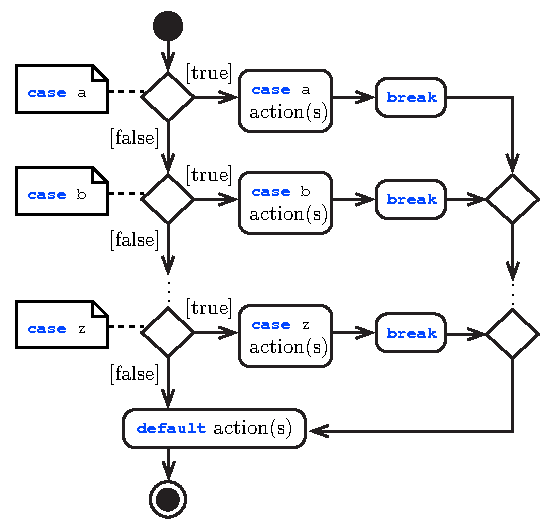
\includegraphics[width=0.75\linewidth]{01_Basics/figures/uml/SelectionStatement-01-UML-switch.pdf}
\captionof{figure}{UML \texttt{switch} \\Activity Diagram Representation}
\label{fig:ch01_Basics_UML_SelStatement-01-switch}
%~\ref{fig:ch01_Basics_UML_SelStatement-01-switch} 
%%%%%%%%%%%%%%%%%%%%%%%%%%End figure
\end{minipage}
\begin{minipage}{.25\textwidth}
%%%%%%%%%%%%%%%%%%%%%%%%%%%%%%%%%Begin code
\begin{CPPCode}
//example
int grade{100};
switch (grade/10)
{
    case 9:
    case 10:
        //¿\codecomment{do smt-1}¿
        break;
    
    case 8:
        //¿\codecomment{do smt-2}¿
        break;
        
    case 7:
    default:
        //¿\codecomment{do-default}¿
        break;
}
\end{CPPCode}
%%%%%%%%%%%%%%%%%%End Code
\end{minipage}
\vspace{0.5cm}
%end minipages



\subsection{Iteration statement}
\subsubsection{\texttt{while}-loop}
%begin minipages
\begin{minipage}{.50\textwidth}
%%%%%%%%%%%%%%%%%%%%%%%%%%%%%%%%%Figure Selection Statement - while
\centering
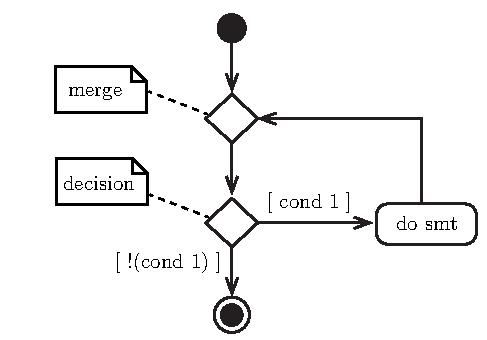
\includegraphics[width=0.80\linewidth]{01_Basics/figures/uml/IterationStatement-00-UML-while.pdf}
\captionof{figure}{UML \texttt{while} \\Activity Diagram Representation}
\label{fig:ch01_Basics_UML_IterationStatement-00-while}
%~\ref{fig:ch01_Basics_UML_IterationStatement-00-while} 
%%%%%%%%%%%%%%%%%%%%%%%%%%End figure
\end{minipage}
\begin{minipage}{.25\textwidth}
%%%%%%%%%%%%%%%%%%%%%%%%%%%%%%%%%Begin code
\begin{CPPCode}
while (cond_1)
{
    //¿\codecomment{do smth}¿
}
\end{CPPCode}
%%%%%%%%%%%%%%%%%%End Code
\end{minipage}
\vspace{0.5cm}
%end minipages

\subsubsection{\texttt{for}-loop}
%begin minipages
\begin{minipage}{.50\textwidth}
%%%%%%%%%%%%%%%%%%%%%%%%%%%%%%%%%Figure Selection Statement - for loop
\centering
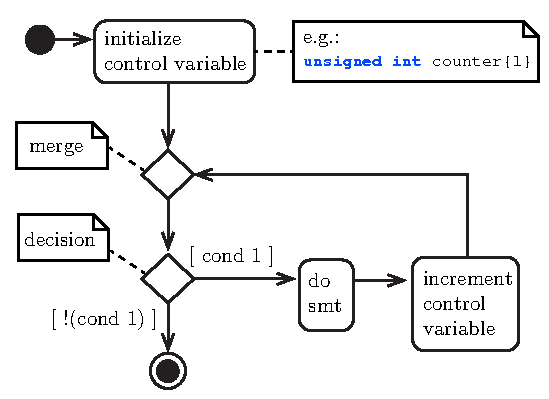
\includegraphics[width=0.80\linewidth]{01_Basics/figures/uml/IterationStatement-01-UML-for.pdf}
\captionof{figure}{UML \texttt{for-loop} \\Activity Diagram Representation}
\label{fig:ch01_Basics_UML_IterationStatement-01-for}
%~\ref{fig:ch01_Basics_UML_IterationStatement-01-for} 
%%%%%%%%%%%%%%%%%%%%%%%%%%End figure
\end{minipage}
\begin{minipage}{.415\textwidth}
%%%%%%%%%%%%%%%%%%%%%%%%%%%%%%%%%Begin code
\begin{CPPCode}
//example-01
for (unsigned int i{10}; i ¿\texttt{>=}¿ 1; i--) 
{...}
//example-02
for (unsigned int i{20}; i ¿\texttt{>=}¿ 2; i -= 2) 
{...}
\end{CPPCode}
%%%%%%%%%%%%%%%%%%End Code
\end{minipage}
\vspace{0.5cm}
%end minipages

\subsubsection{\texttt{do-while}-loop}
%begin minipages
\begin{minipage}{.55\textwidth}
%%%%%%%%%%%%%%%%%%%%%%%%%%%%%%%%%Figure Selection Statement - do-while
\centering
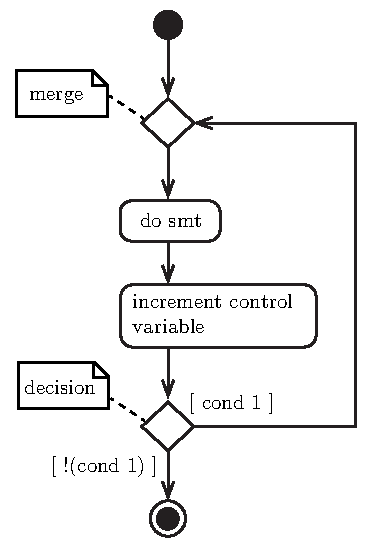
\includegraphics[width=0.58\linewidth]{01_Basics/figures/uml/IterationStatement-02-UML-do-while.pdf}
\captionof{figure}{UML \texttt{do-while-loop} \\Activity Diagram Representation}
\label{fig:ch01_Basics_UML_IterationStatement-01-for}
%~\ref{fig:ch01_Basics_UML_IterationStatement-01-for} 
%%%%%%%%%%%%%%%%%%%%%%%%%%End figure
\end{minipage}
\begin{minipage}{.25\textwidth}
%%%%%%%%%%%%%%%%%%%%%%%%%%%%%%%%%Begin code
\begin{CPPCode}
//example:
unsigned int counter{1}
do
{
    //¿\codecomment{do smt}¿
    ++counter;
} while (counter <= 10)
\end{CPPCode}
%%%%%%%%%%%%%%%%%%End Code
\end{minipage}
\vspace{0.5cm}
%end minipages


%code comment:
% ¿\codecomment{
% no numbers listing
% \begin{lstlisting}[frame=tlrb,numbers=none,mathescape=true,escapechar=\%,columns=flexible]

% \begin{minipage}{.9\textwidth}
% \begin{lstlisting}[frame=tlrb,showlines=htrue,firstnumber=1,mathescape=true,escapechar=\%,columns=flexible]
% //code here
% \end{lstlisting}
% \end{minipage}

% \begin{lstlisting}[frame=tlrb,showlines=htrue,firstnumber=1,mathescape=true,escapechar=\%,columns=flexible]
% //Program 12.1
% \end{lstlisting}
    
%reference:
%~\ref{tab:t_ch11_UART_Registers} tab:t_ch12_edgeTriggeredModes
%~\ref{fig:RT_ch01} 
%\texttt{Ascii}
%\texttt{UART}
%\texttt{mailbox}
%\texttt{FIFO}
%\texttt{I/O}
%\underline{}
%$\texttt{b}_0$
%\sim = ~

%percent
%n%\%%10;

%for loops
% \newcounter{nnCount}
% \forloop{nnCount}{0}{\value{nnCount}<8}{&IME }  
% \forloop{nnCount}{0}{\value{nnCount}<8}{&PMC\arabic{nnCount} }


%Equation array
% \begin{eqnarray*}
%  & = & \text{minimun}\\
%  & = & \text{maximun}\\
%  & = &  \\
%  & = & \\
%  & = & 
% \end{eqnarray*}

% \begin{description}
% \item[Remark 1] If
% \end{description}

% \begin{description}
% \item[Remark 1] If
% \item[Remark 2] An
% \item[Remark 3] With 
% \end{description}

%Poner figura
% \begin{figure}[!h] %%%%%%%%%%%%%%%%%%%%%%% Begin Figure Directory
% \centering
% \includegraphics[width=0.70\linewidth]{figuresRT/ch06/RT-CH06-
% \caption{Free-space management.}
% \label{fig:ch01_00}
% %~\ref{ffig:ch01_00} 
% \end{figure}       %%%%%%%%%%%%%%%%%%%%%%% End Figure

%Poner Figura con minipages
% %begin minipages
% \begin{minipage}{.45\textwidth}
% %here some text.
% \end{minipage}
% \begin{minipage}{.55\textwidth}
% %and here the image.
% \centering
% \includegraphics[width=0.95\linewidth]{figures/ch12/ch12_lab12_squeme1.pdf}
% \captionof{figure}{Lab 12 diagram connections}
%\label{fig:RT_ch04_MACQ-EXAMPLE-01-oldDataIsLost}
%~\ref{fig:RT_ch04_MACQ-EXAMPLE-01-oldDataIsLost} 
% \end{minipage}
% \vspace{0.5cm}
% %end minipages

% %Poner Figura y al costado codigo
% %begin minipages
% \begin{minipage}{.60\textwidth}
% %%%%%%%%%%%%%%%%%%%%%%%%%%%%%%%%%Figure Selection Statement - while
% \centering
% 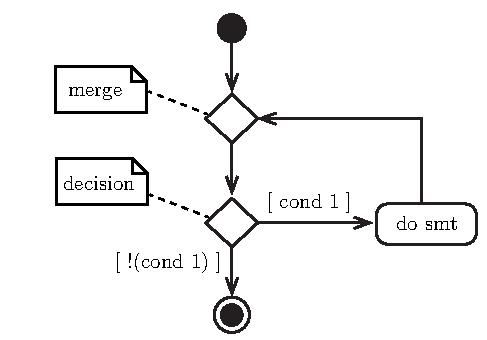
\includegraphics[width=0.50\linewidth]{01_Basics/figures/uml/IterationStatement-00-UML-while.pdf}
% \captionof{figure}{UML \texttt{while} Activity Diagram Representation}
% \label{fig:ch01_Basics_UML_IterationStatement-00-while}
% %~\ref{fig:ch01_Basics_UML_IterationStatement-00-while} 
% %%%%%%%%%%%%%%%%%%%%%%%%%%End figure
% \end{minipage}
% \begin{minipage}{.25\textwidth}
% %%%%%%%%%%%%%%%%%%%%%%%%%%%%%%%%%Begin code
% \begin{lstlisting}[frame=tlrb,numbers=none,mathescape=true,escapechar=\%,columns=flexible]
% some awesome code here
% \end{lstlisting}
% %%%%%%%%%%%%%%%%%%End Code
% \end{minipage}
% \vspace{0.5cm}
% %end minipages


%\begin{enumerate}
%	\item Initialize timer and directions registers
%    \item Specify initial state
%    \item Perform FSM controller
%   \begin{enumerate}
%    	\item Call an output function, which depends on the state
%        \item Delay, which depends on the state
%        \item Call an input function to get the status of the coin sensors
%        \item Change states, which dependes on the state and the input
%    \end{enumerate}
%\end{enumerate}

% \begin{enumerate}
% 	\item Current instruction is finished,
%     \item Eight registers are pushed on the stack,
%     \item LR is set to 0xFFFFFFF9,
%     \item IPSR is set to the interrupt number,
%     \item PC is loaded with the interrupt vector
% \end{enumerate}

% Itemize categoriza poniendo (.) en lugar de números
% \begin{itemize} 
% 	\item I
% 	\item I
% 	\item Y
% 	\item Y
% 	\item Y
% 	\item Y
% 	\item 
% \end{itemize}

% \begin{table}[!h]
% \centering
% \begin{tabular}{|l|l|l|} \hline
% $p$ & bit Field & Interrupt         \\\hline
% $3$ & \bitsRange[31]{29} & Interrupt [$4m+3$]  \\\hline
% $2$ & \bitsRange[23]{21} & Interrupt [$4m+2$]  \\\hline
% $1$ & \bitsRange[15]{13} & Interrupt [$4m+1$]  \\\hline
% $0$ & \bitsRange[7]{5} & Interrupt [$4m$]   \\\hline
% \end{tabular}
% \caption{pasteCaption}
% \label{tab:t_rt_ch04_}
% ~\ref{tab:t_rt_ch04_}
% \end{table}

% Insertar URL
%\url{https://www.osha.gov/Publications/laboratory/OSHAfactsheet-laboratory-safety-noise.pdf}\\

% \newcommand{\bitsRange}[2][50]{\texttt{{#1}-{#2}}}
% \newcommand{\CustomHex}[2][0000]{\texttt{0x{#1}.{#2}}}
% \newcommand{\GPIOPort}[1]{\texttt{GPIO\_PORT{#1}}}
% \newcommand{\GPIOPortR}[2][A]{\texttt{GPIO\_PORT{#1}\_{#2}\_R}}
% \newcommand{\GPIOPortHandler}[1]{\texttt{GPIO\_PORT{#1}\_Handler}}
% \newcommand{\HandlerISR}[1]{\texttt{#1\_Handler}}
% \newcommand{\IRQnr}[1]{\texttt{{#1}}}
% \newcommand{\NVICPRI}[1]{\texttt{NVIC\_PRI{#1}\_R}}
% \newcommand{\NVICEN}[1]{\texttt{NVIC\_EN{#1}\_R}}
% \newcommand{\NVICDIS}[1]{\texttt{NVIC\_DIS{#1}\_R}}
% \newcommand{\Ttimer}[2][A]{\texttt{Timer\_{#2}{#1}}}
% \newcommand{\xNrbit}[1]{$#1$-\texttt{bit}}
% \newcommand{\xNrbits}[1]{$#1$-\texttt{bits}}
% \newcommand{\camouflagegreenCellColor}{\cellcolor[rgb]{0.47, 0.53, 0.42}}
% \newcommand{\lavenderCellColor}{\cellcolor[rgb]{0.9, 0.9, 0.98}}
% \newcommand{\volties}[2][0]{$\si{{#1}\volt}_{#2}$}
% \newcommand{\volti}[1]{$\si{{#1}\volt}$}
% \newcommand{\voltiposi}[1]{$+\si{{#1}\volt}$}
% \newcommand{\voltinega}[1]{$-\si{{#1}\volt}$}
\newpage
%chapter*{\glossarytitlename}
\addcontentsline{toc}{chapter}{Abbreviations}
\begin{acronym}[ABCDEFGHIJK]
%A
\acro{API}{Application Programming Interface} %\ac{API}
\acro{APB}{Advanced Peripheral Bus} %\ac{APB}
%D
\acro{DAE}{Differential-Algebraic Equation}
\acro{DDI}{Differential Dissipativity Inequality}%\ac{DDI} 
\acro{DOF}{Degrees of Freedom}
%E
\acro{ES}{Energy Shaping}
%I
\acro{ISR}{Interrupt Service Routine} %\ac{ISR}
%P
\acro{PBC}{Passivity Based Control}
\acro{PDE}{Partial Differential Equation}
\acro{PFL}{Partial Feedback Linearization}
\acro{pH}{port-Hamiltonian}
%R
\acro{RTOS}{Real Time Operating System} %\ac{RTOS}
%S
\acro{SMC}{Sliding Mode Control}
\acro{SysML}{System Modelling Language} % \ac{UMS}
%U
\acro{UMS}{Underactuated Mechanical System} % \ac{UMS}
\acro{UML}{Unified Modelling Language} % \ac{UMS}
%Z

\end{acronym}
\clearpage

\bibliographystyle{IEEEtran}
\bibliography{myReferences}
\end{document}
